\subsection{Long term speckle pulsing}\label{long_pulse}

In the experiments, it is important to know the average speckle potential at the atoms. But unfortunately, it is hard to measure the power of the speckle beam directly at the atoms and infer the average speckle potential. Because in the experiments, we can not put a power meter anywhere we want to measure the power of the beam. And besides, it is the intensity that matters, and we don't have perfect knowledge of the beam size at the atoms. After the closest point to the vacuum glass cell where we can use a power meter to measure the power, the beam goes through lenses, reflected by mirrors, glass cell or even dichroic mirrors. The power of the beam decreases at each of the optical element. To the best of our knowledge, for the previous experiments using speckle beams, the average speckle potential was not measured directly. It could be inferred by calculating the power given the power loss at each optical element. Or the power could be measured for an identical speckle beam set up on the test bench and it is assumed the power at the atoms is the same as the power of the test speckle beam in the focal plane. 

Inspired by \cite{huckans2009quantum}, we obtained the mean potential depth by making the atoms evolve under the speckle beam pulses. Compared with \cite{huckans2009quantum}, for $t \gg t_{RN}$, we do not expect to see the collapse and revive phenomenon due to the anharmonicity of the speckle potential. Instead, at long speckle pulsing time, the momentum distribution should reach equilibrium and by virial theorem, the average stationary kinetic energy is half of the average total energy which is the initial average speckle potential. 

To confirm our understanding, we did numerical simulations of the long-term speckle pulsing. Fig.~\ref{fig:speckle_pulsing} shows the simulation and experimental results of the speckle pulsing for the pulsing duration up to $2\ {\rm ms}$. In the simulation, we release the BECs from the dipole trap and immediately turn on the speckle potential. The atoms evolve under the speckle potential and we keep track of the width of the momentum distribution. We did the simulation for different average speckle potential depth ranging from $0\ {\rm Hz}$ to $1600\ {\rm Hz}$, with a $200\ {\rm Hz}$ spacing. The results are shown as the nine curves, each one is averaged over 20 speckle realizations. When the average speckle potential is zero, the width of the momentum distribution increases driven by the mean-field expansion. From the simulation results shown in Fig.~\ref{fig:speckle_pulsing}(a), the width of the momentum distribution increases rapidly after the speckle potential is turned on and becomes stationary after around $0.25\ {\mu s}$. The stationary width increases with the average speckle potential depth. Fig.~\ref{fig:speckle_pulsing}(b) shows the experimental results. In the experiment, we release the atoms from the dipole trap, pulse the speckle potential for up to $2\ {\rm mm}$ followed by TOF. The total time for the speckle pulsing and the TOF is $18\ {\rm ms}$, a constant for different pulsing duration. We take the absorption images after TOF and fit a Gaussian function to the density profile of the atoms. Fig.~\ref{fig:speckle_pulsing}(b) shows the width of the fitted Gaussian function vs the duration of the speckle pulses. The Gaussian width increases with the pulsing duration in short term and becomes stationary after around $0.25\ {\rm ms}$, which is consistent with the simulation results. 

\begin{figure*}
    \centering
    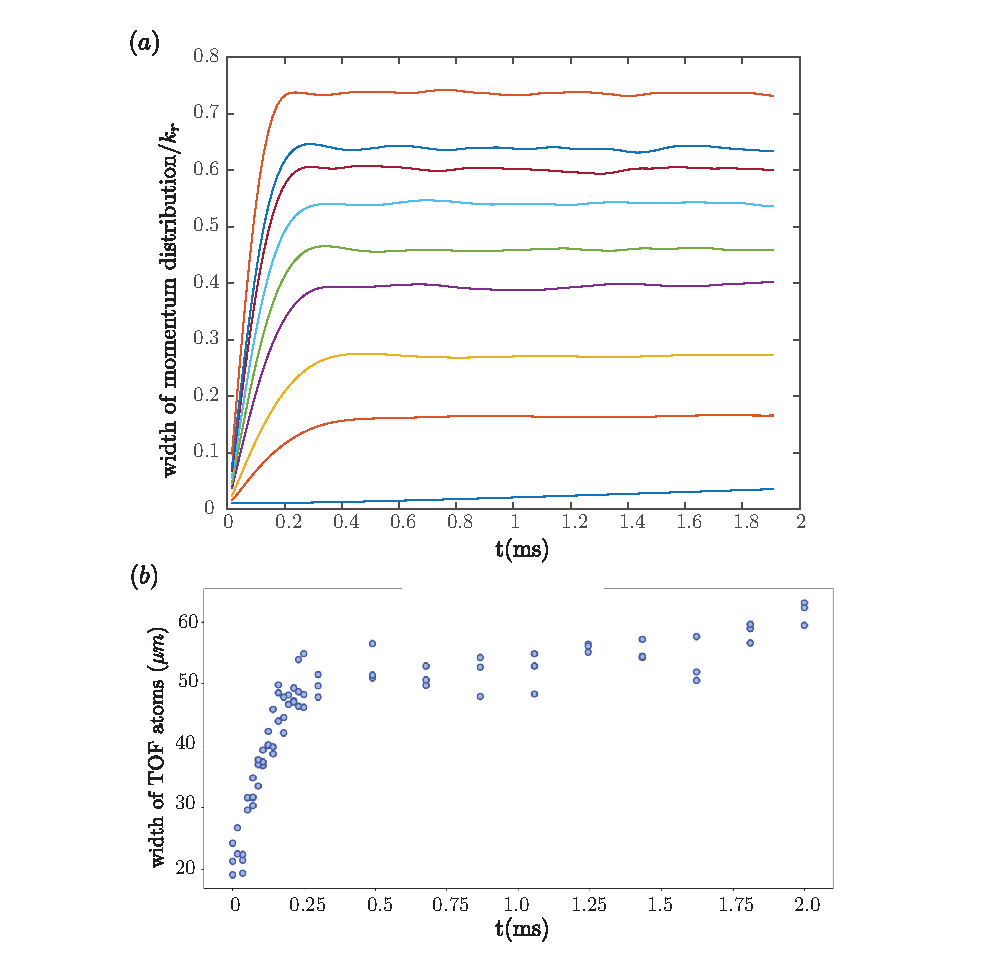
\includegraphics{Chapter6_secs/speckle_pulsing_width.pdf}
    \caption{The simulation and the experiments of the speckle beam pulsing. (a). The width of the momentum distribution of atoms evolving under the speckle potentials of different potential depth ranging from $0$ to $1600\ {\rm Hz}$.  (b). The Gaussian width of atoms in the absorption images after TOF for different speckle pulsing duration.}
    \label{fig:speckle_pulsing}
\end{figure*}

To infer the average speckle potential from the width of the momentum distribution after long-term speckle pulsing, we compute the average kinetic energy using the fitted Gaussian width of the density profile of atoms after TOF.
\begin{equation}
    \langle \hat{K} \rangle = \frac{1}{2} m \left(\frac{\sigma}{\tau}\right)^2
\end{equation}
Here $\tau$ is the time for TOF. The average speckle potential is equal to the average total energy, which by virial theorem is twice the average kinetic energy. In Fig.~\ref{fig:avg_speckle_poten}(b), the computed total energy is plotted against a photo diode (PD) reading. In our experiments, we use a pick-off mirror to reflect a fixed percentage of the power of the speckle beam to a PD and the reading of the PD in Volt is proportional to the power of the beam at the atoms. We fit a line crossing the origin to the data, by reading the PD we have an estimate of the average speckle potential at the atoms. 

To compare with the experimental results, we also did numerical simulations. In the simulations, we release the atoms from the dipole trap at $t=0$ and pulse the speckle potential for $1\ {\rm ms}$ followed by a $20\ {\rm ms}$ free evolution. The simulations are done with two kinds of speckle potentials, $k_c=0.80k_r$ and $k_c=1.48k_r$, respectively. For each kind of the speckle potential, the average potential depth ranges from $0\ {\rm Hz}$ to $1600\ {\rm Hz}$ with a $200\ {\rm Hz}$ spacing. We compute the momentum distribution and the average kinetic energy at the end of the free evolution. The average total energy is twice the average kinetic energy deducted by the mean-field energy computed from the average kinetic energy in the no-pulsing case. And the resultant average total energy is plotted against the known average potential depth. In agreement with our prediction, the curves are close to the diagonal line (dashed) for both kinds of speckle potentials.


\begin{figure*}
    \centering
    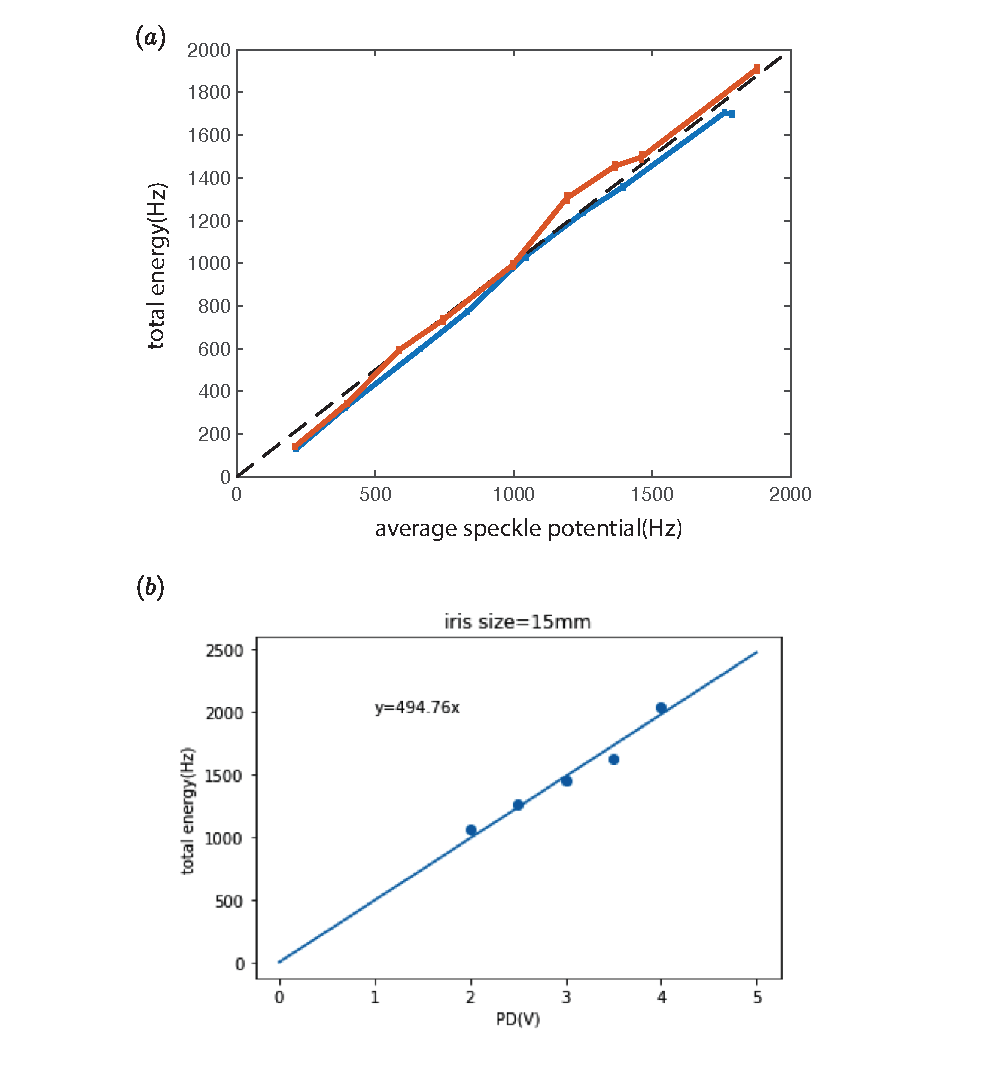
\includegraphics{Chapter6_secs/average_speckle_potential.pdf}
    \caption{Calibration of the average speckle potential depth. (a). In the numerical simulation, the average total energy inferred from the momentum distribution after $20\ {\rm ms}$ free evolution is plotted against the known average speckle potential depth. The red curve and the blue curve are for the speckle potentials with $k_c = 0.80k_r$ and $k_c=1.48k_r$, respectively. The dashed line is diagonal. (b). In the experiment, the average total energy computed from long-term speckle pulsing data is plotted against the PD reading.}
    \label{fig:avg_speckle_poten}
\end{figure*}



